\part{Results}

This chapter presents the relevant results of the investigation and experimentation phases.
Presenting the tested cloud container orchestration platforms first,
followed by the results per metric requirement thereafter.

\chapter{Results}

\section{Viable Solutions}
The following platforms were evaluated as potential solutions:
\begin{itemize}
  \item AWS Lambda (representing \textit{Serverless Functions})
  \item AWS ECS (representing \textit{Cloud Native})
        \begin{itemize}
          \item running on EC2 (representing \textit{Virtual Machines})
          \item running on Fargate (representing \textit{Serverless Containers})
        \end{itemize}
  \item AWS EKS (representing \textit{Kubernetes})
        \begin{itemize}
          \item running on EC2 (representing \textit{Virtual Machines})
          \item running on Fargate (representing \textit{Serverless Containers})
        \end{itemize}
\end{itemize}

\section{Experimentation Results}

\begin{figure}[hp]
  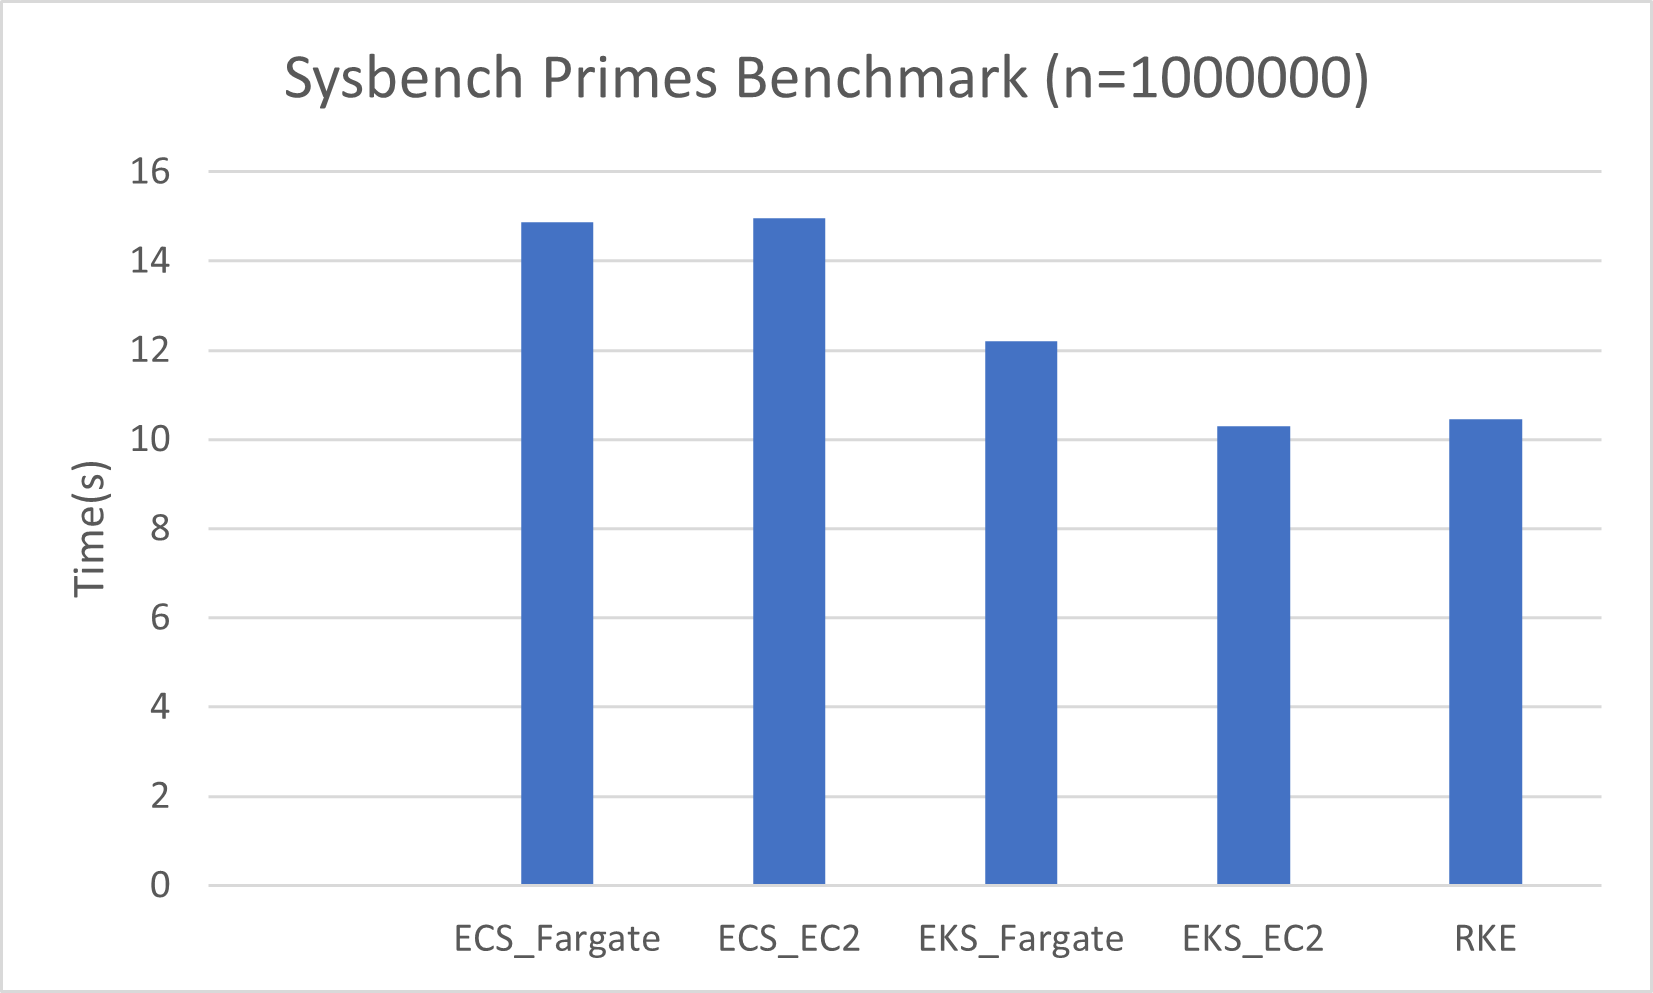
\includegraphics{images/perf-sysbench.png}
  \caption{\emph{Performance}: Average time taken to compute primes up to 1000000 }
  \label{fig:perf_sysbench}
\end{figure}

\begin{figure}[hp]
  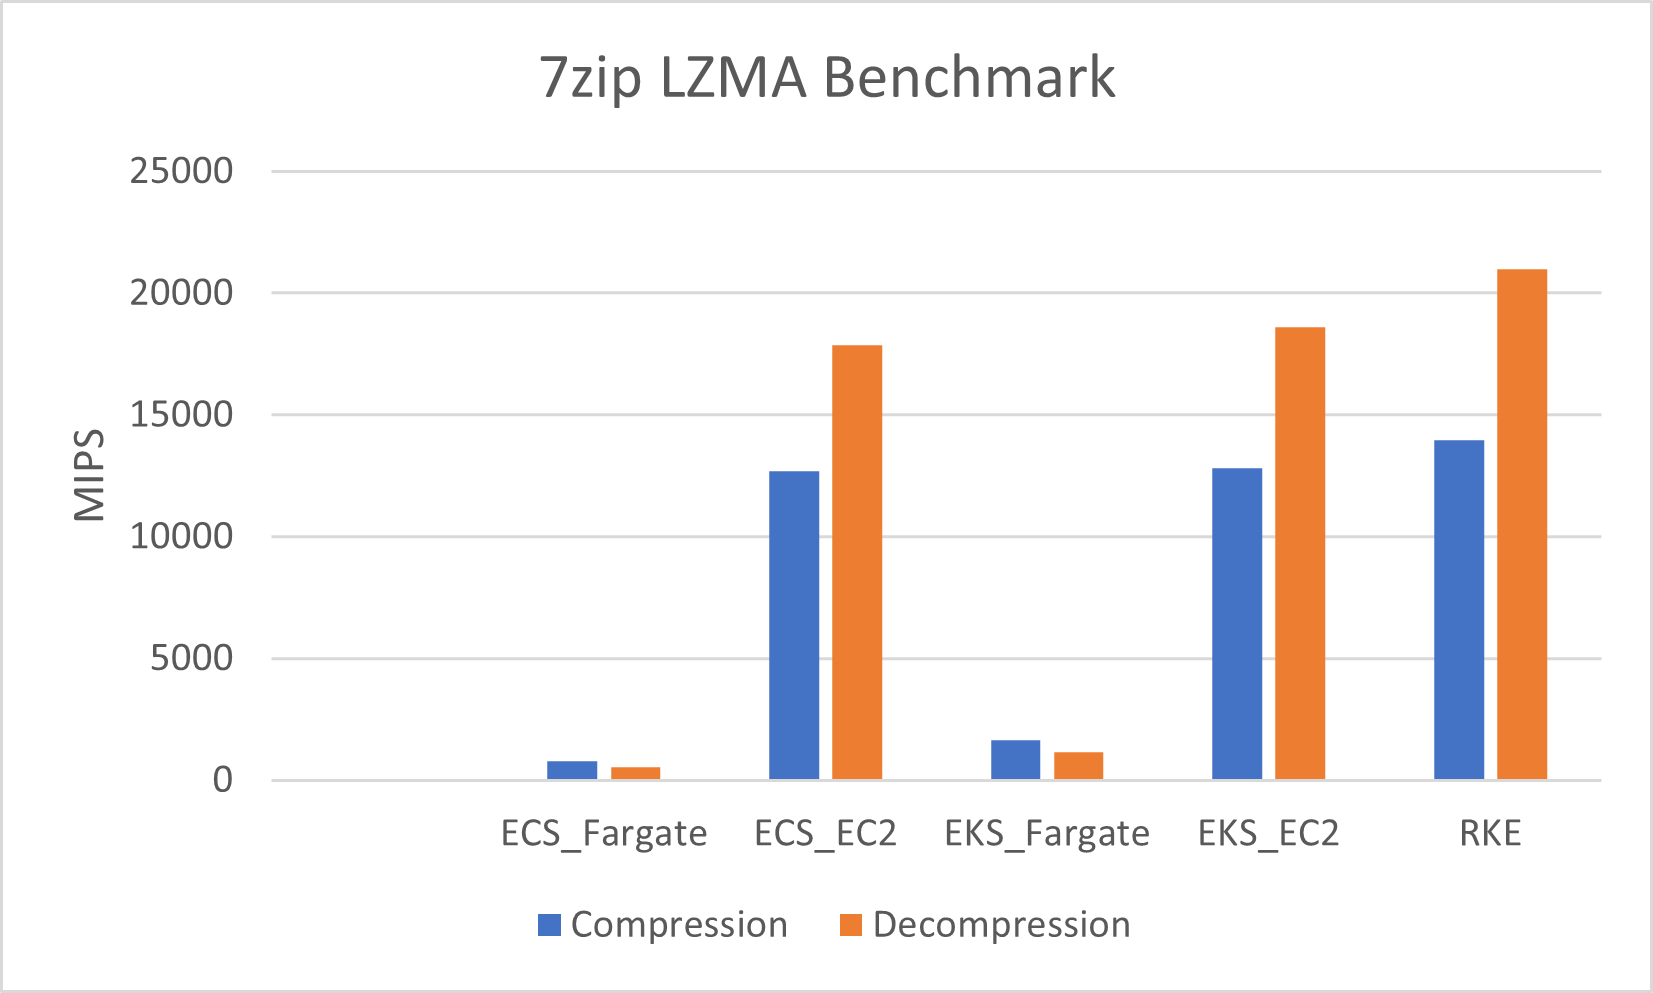
\includegraphics{images/perf-7zip.png}
  \caption{\emph{Performance}: Average rating in MIPS to complete the 7zip LZMA Benchmark }
  \label{fig:perf_7zip}
\end{figure}

\begin{figure}[hp]
  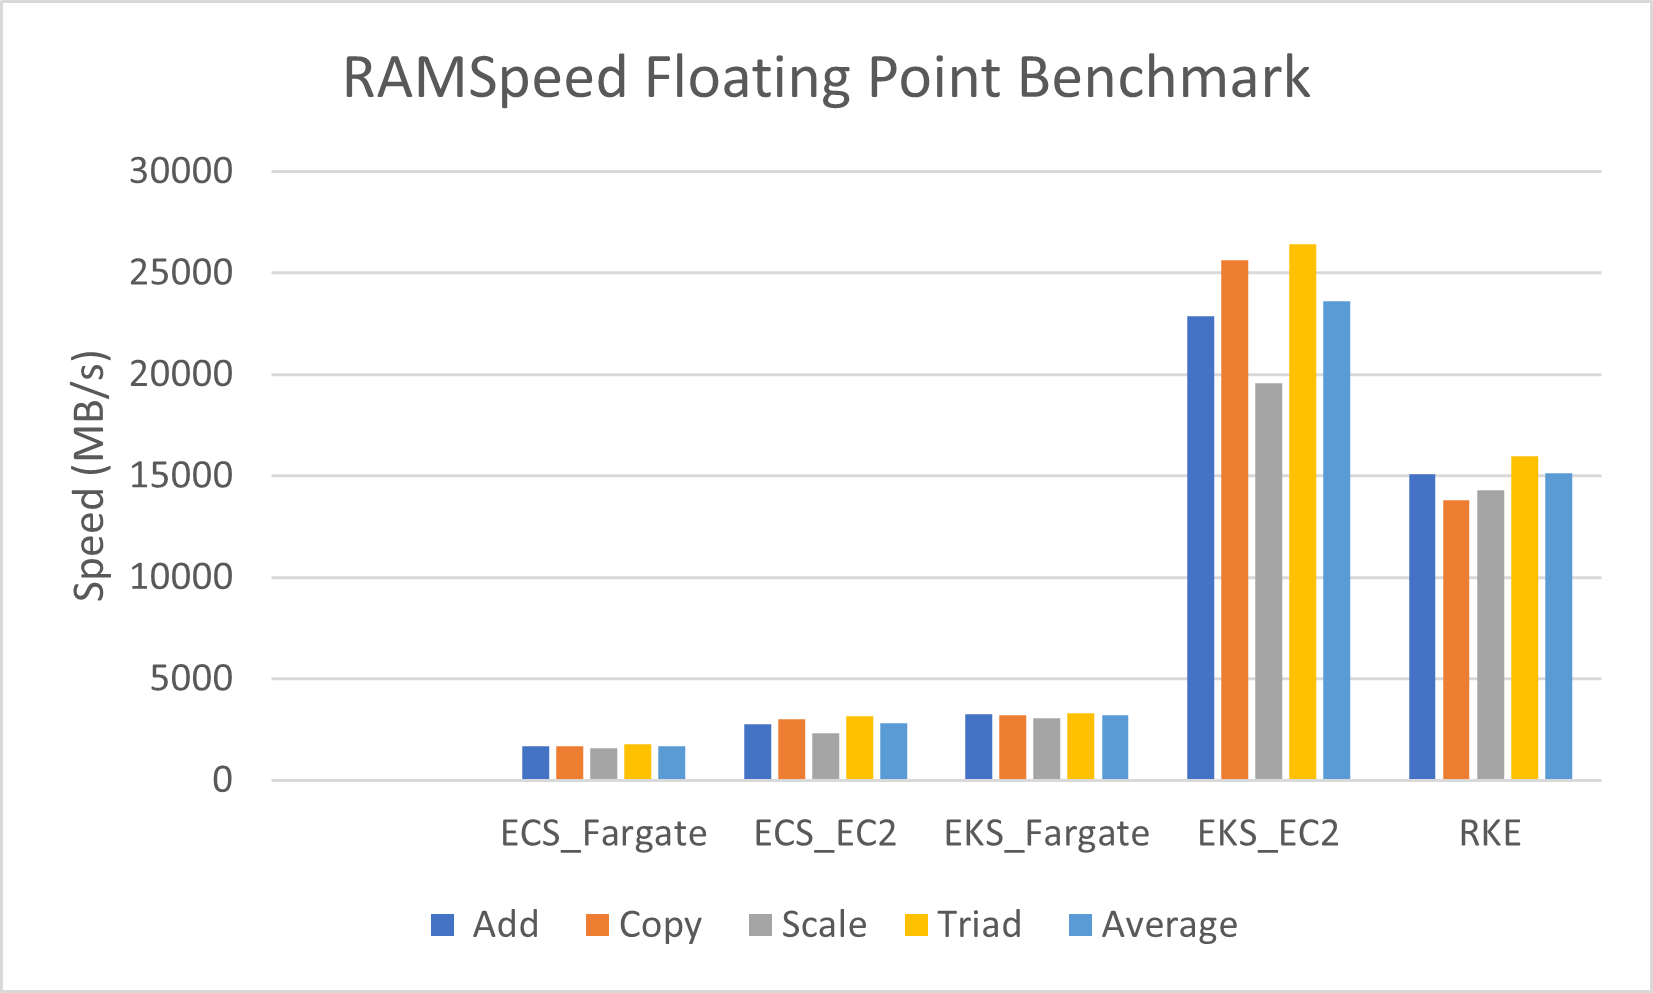
\includegraphics{images/perf-RAMSpeed.png}
  \caption{\emph{Performance}: Average maximum speed achieved whilst completing the RAMSpeed Benchmark }
  \label{fig:perf_RAMSpeed}
\end{figure}

\begin{figure}[hp]
  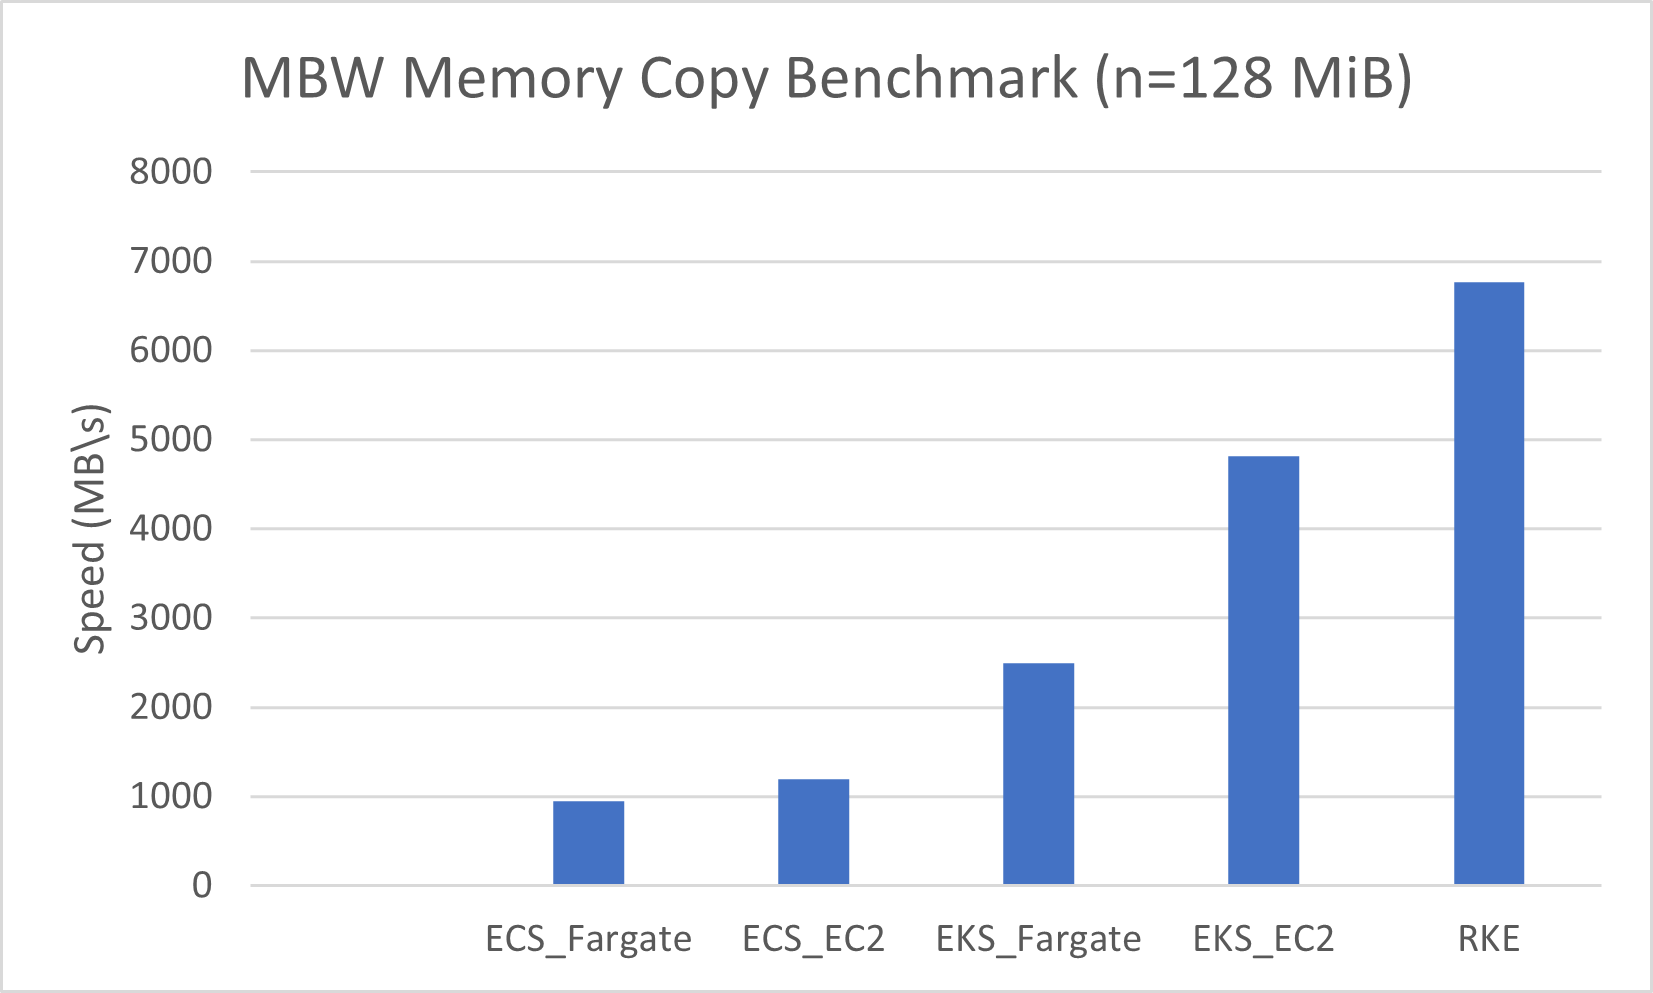
\includegraphics{images/perf-MBW.png}
  \caption{\emph{Performance}: Average maximum speed achieved whilst completing the Memory Bandwidth Benchmark }
  \label{fig:perf_MBW}
\end{figure}

\begin{figure}[hp]
  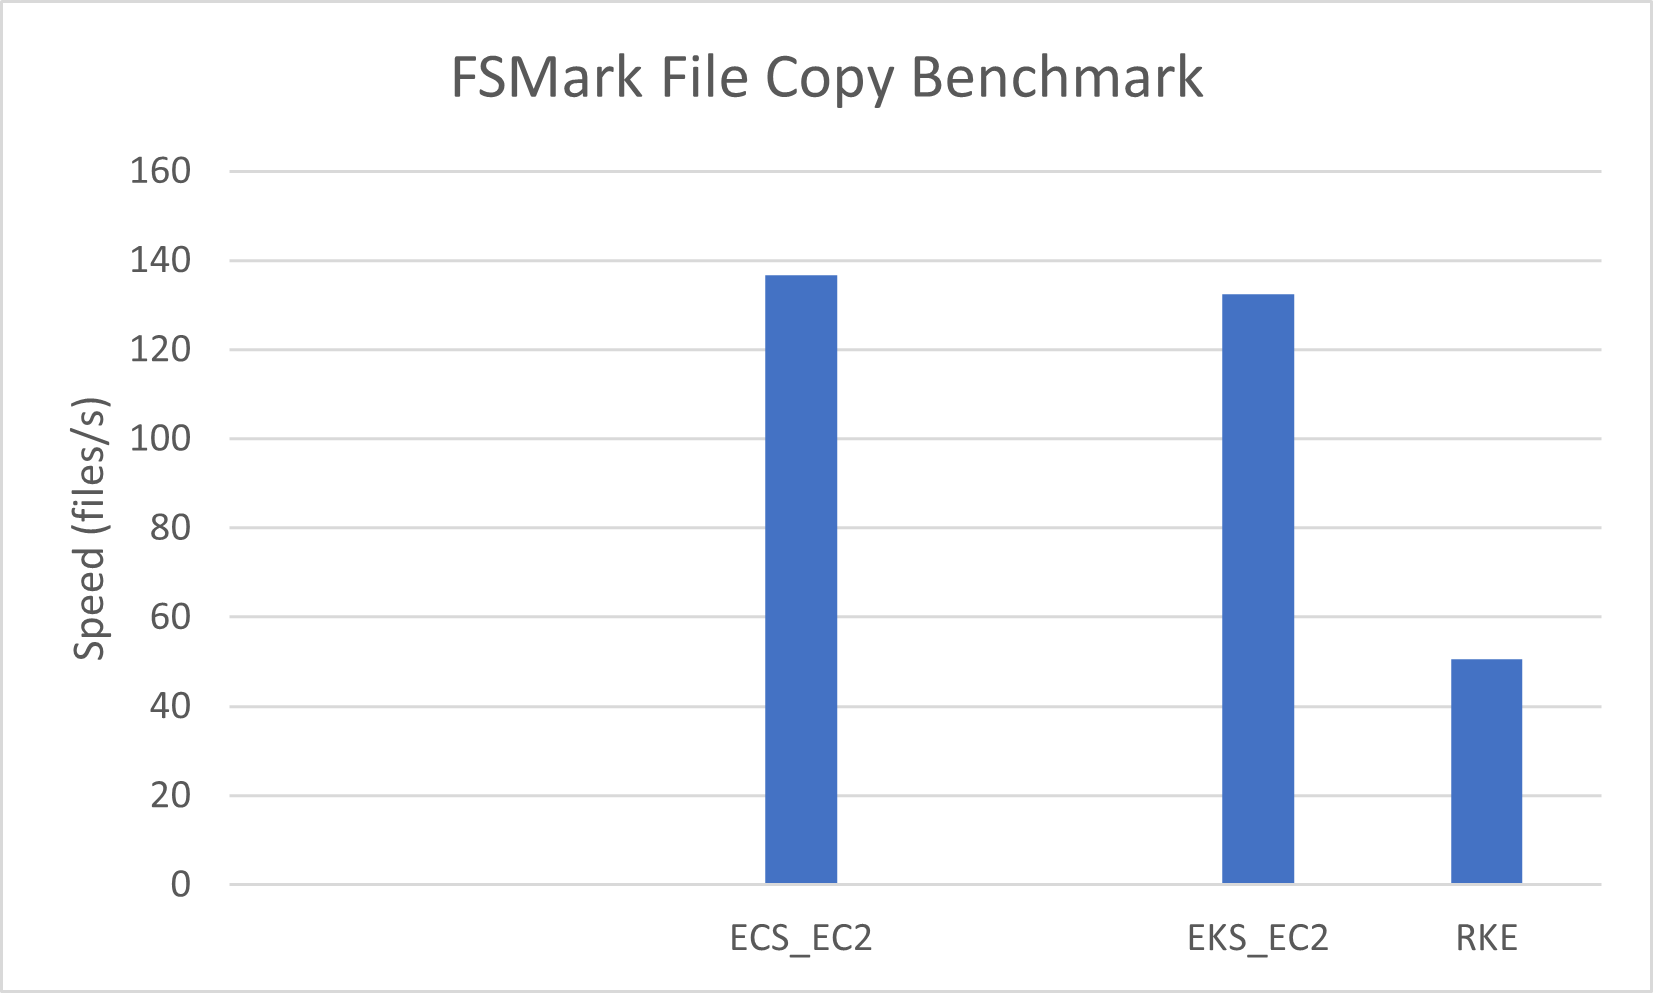
\includegraphics{images/perf-FSMark.png}
  \caption{\emph{Performance}: Average maximum speed achieved whilst completing the fs\_mark Benchmark }
  \label{fig:perf_FSMark}
\end{figure}

\begin{figure}[hp]
  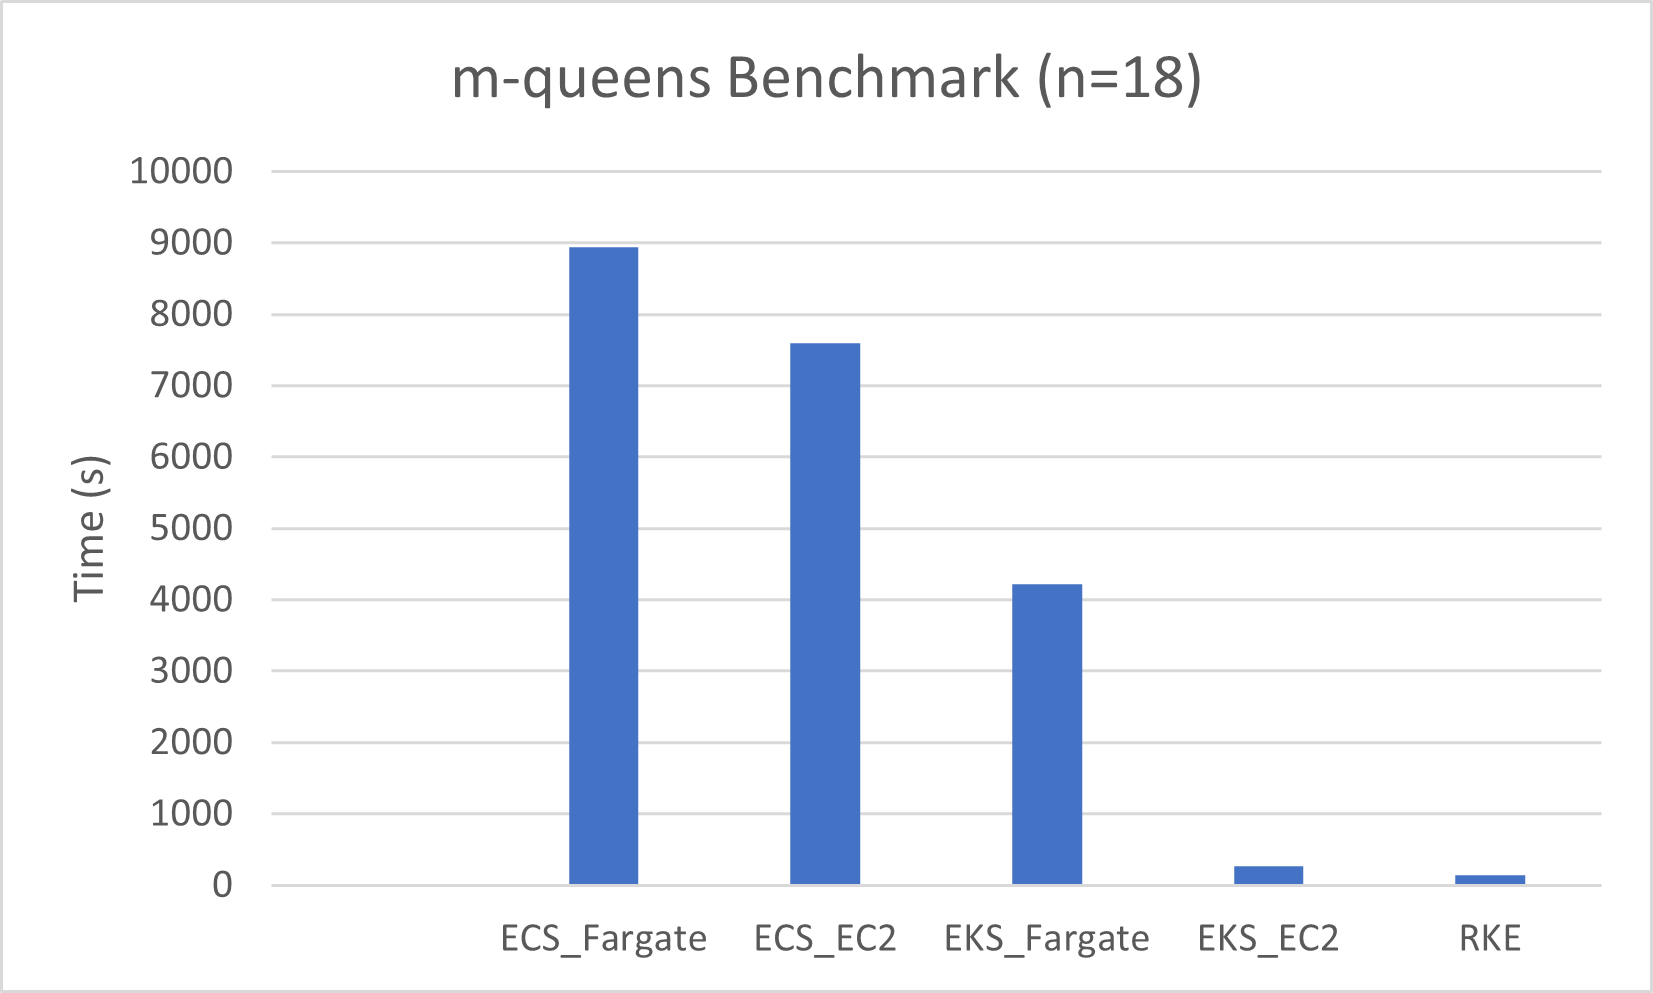
\includegraphics{images/perf-m_queens.png}
  \caption{\emph{Performance}: Average amount of time required to solve the n-queens problem (n=18) }
  \label{fig:perf_mQueens}
\end{figure}

\begin{figure}[hp]
  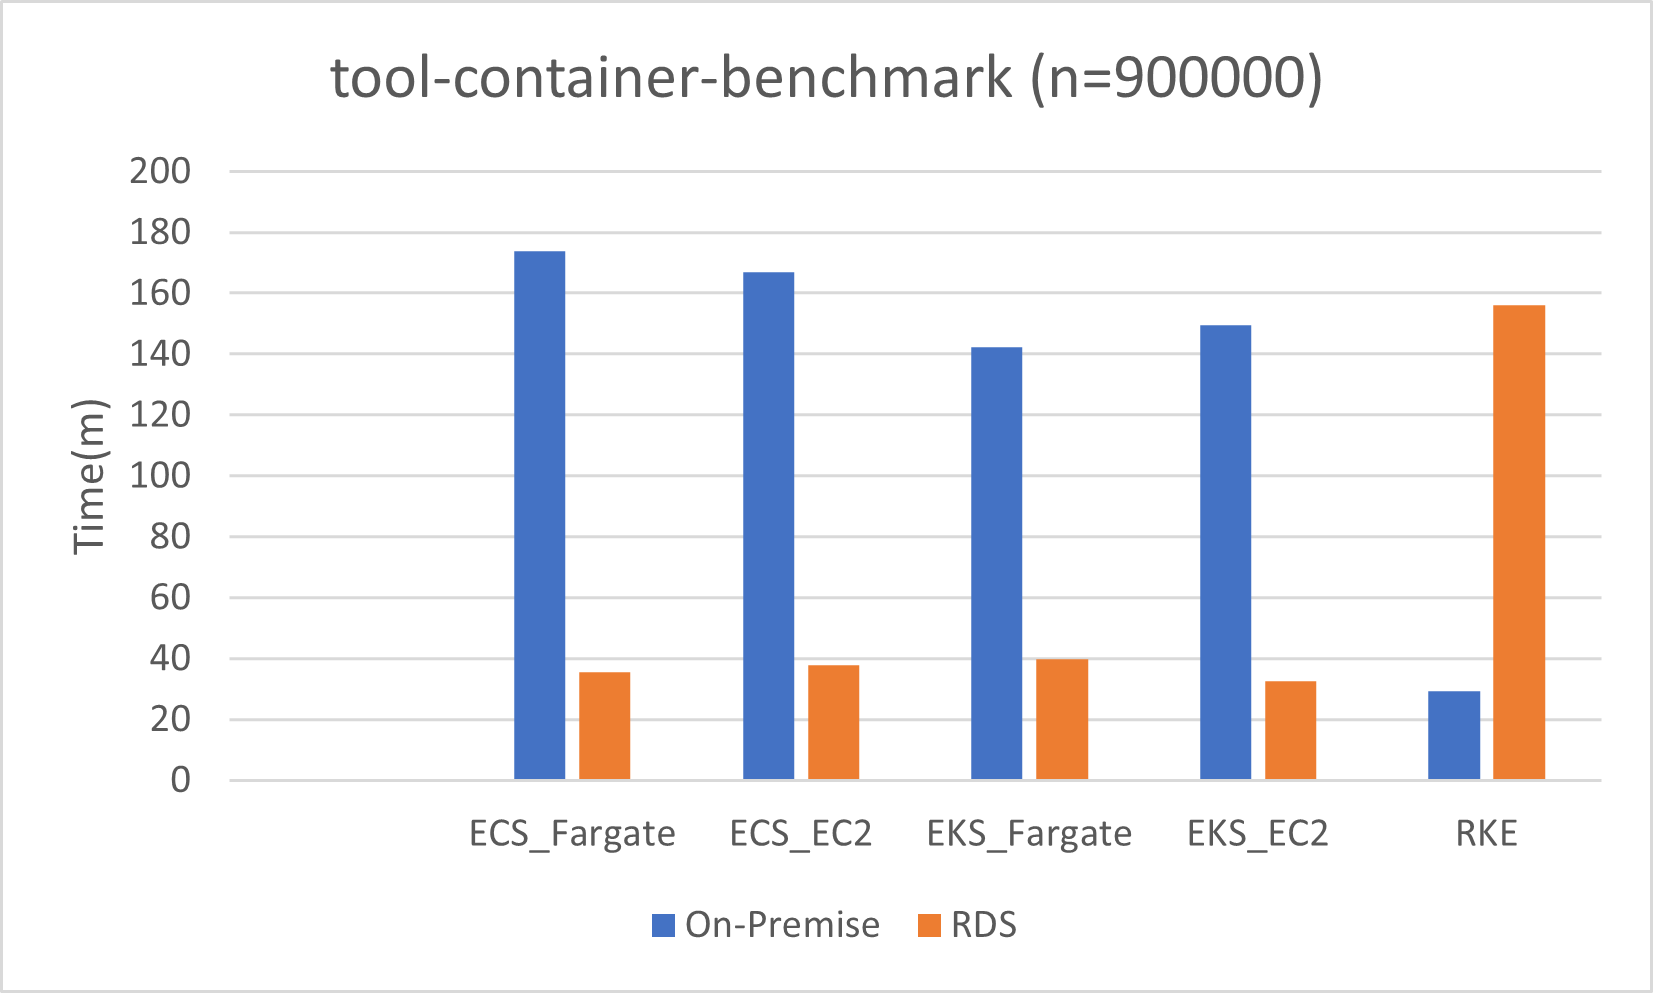
\includegraphics{images/perf-tcb_default.png}
  \caption{\emph{Performance}: Average amount of time required to complete tool-container-benchmark (number\_of\_events=9000000) }
  \label{fig:perf_tcb_default}
\end{figure}

\begin{figure}[hp]
  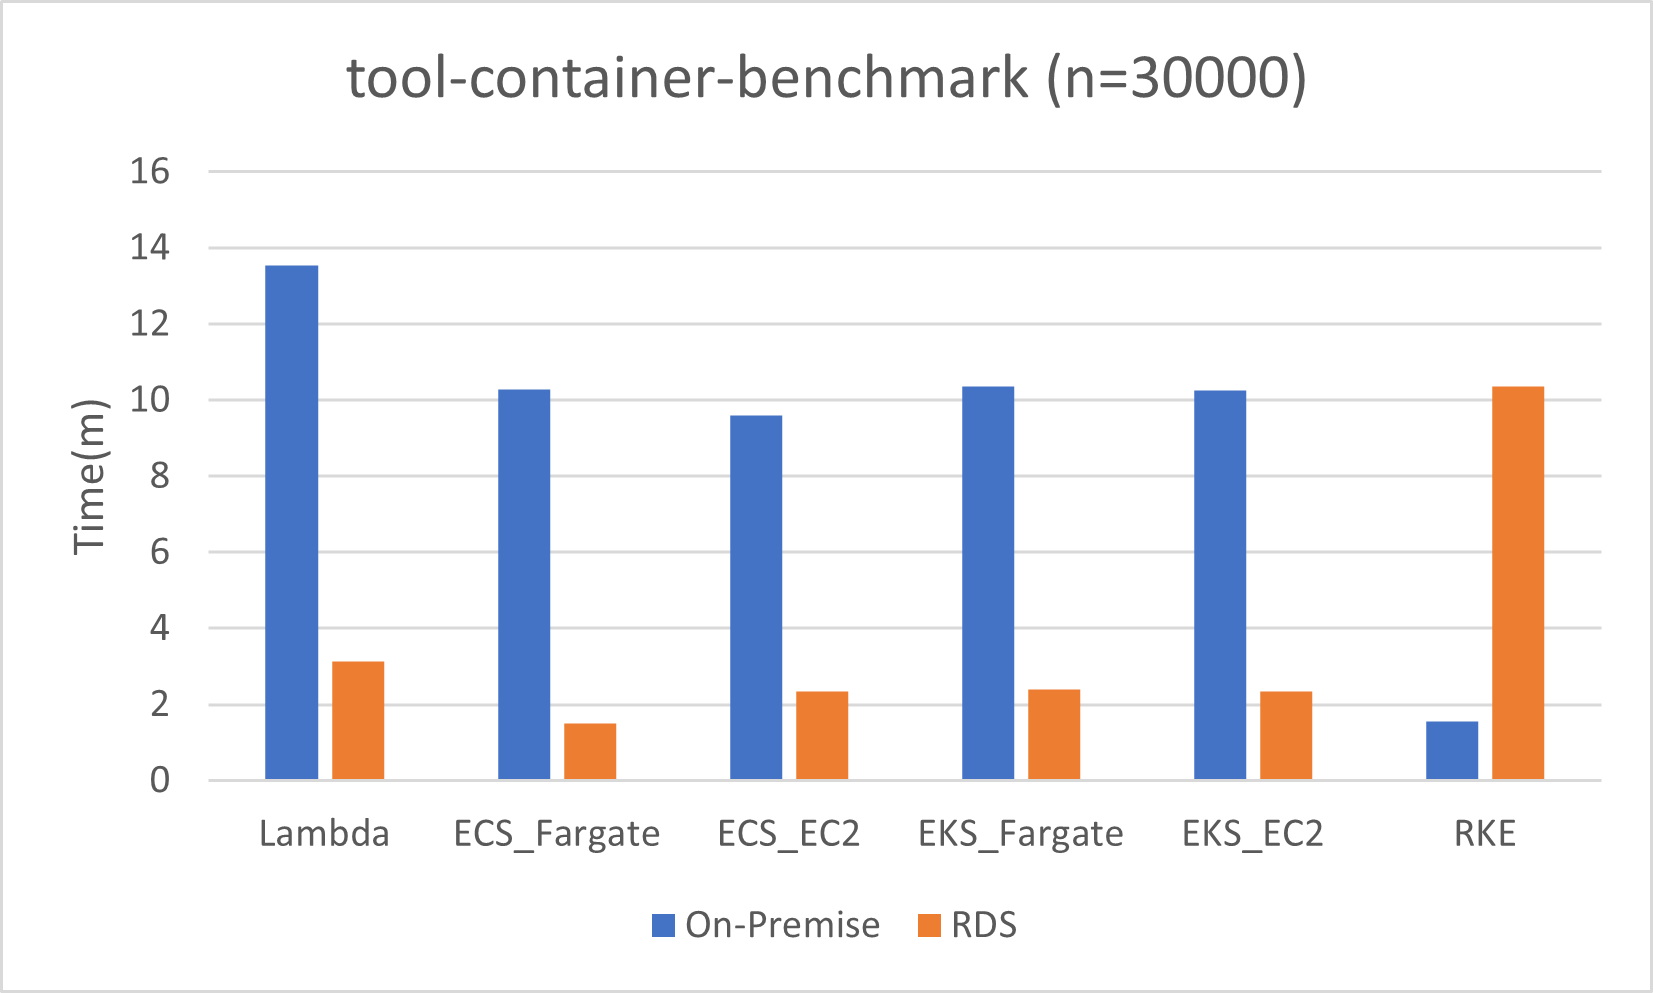
\includegraphics{images/perf-tcb_30000.png}
  \caption{\emph{Performance}:Average amount of time required to complete tool-container-benchmark (number\_of\_events=30000) }
  \label{fig:perf_tcb_30000}
\end{figure}

\begin{figure}[hp]
  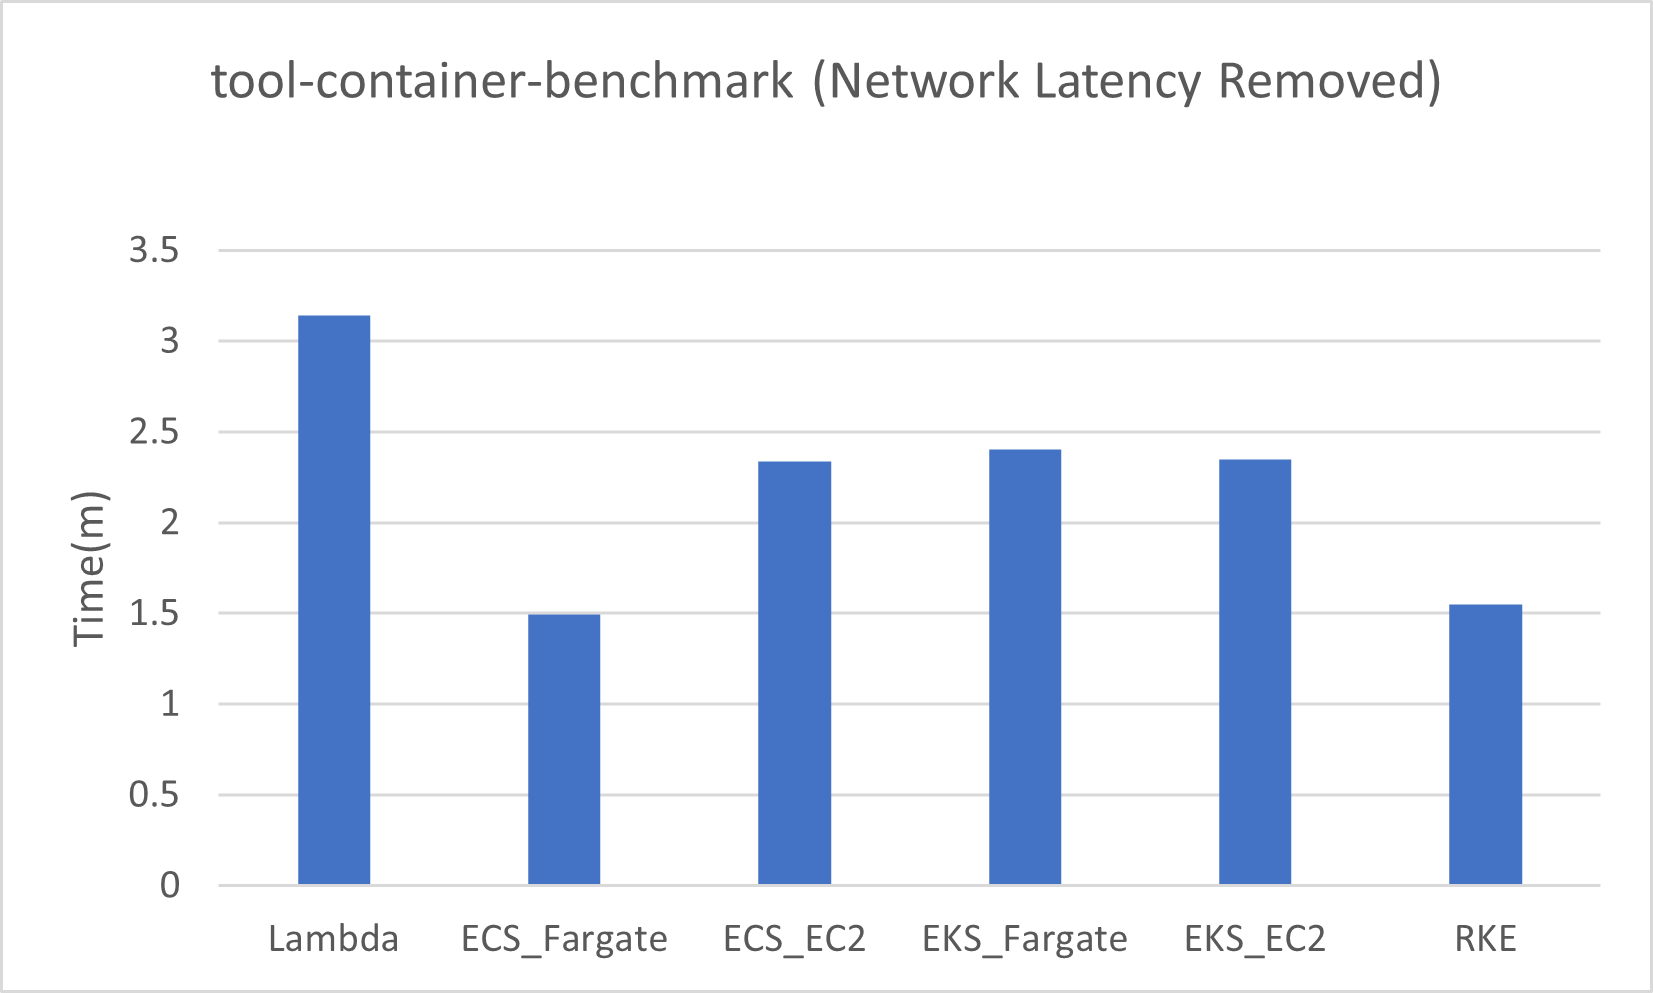
\includegraphics{images/perf-tcb_network.png}
  \caption{\emph{Performance}:Average amount of time required to complete tool-container-benchmark, measured against Database closest to instance (number\_of\_events=30000)}
  \label{fig:perf_tcb_network}
\end{figure}

\begin{figure}[hp]
  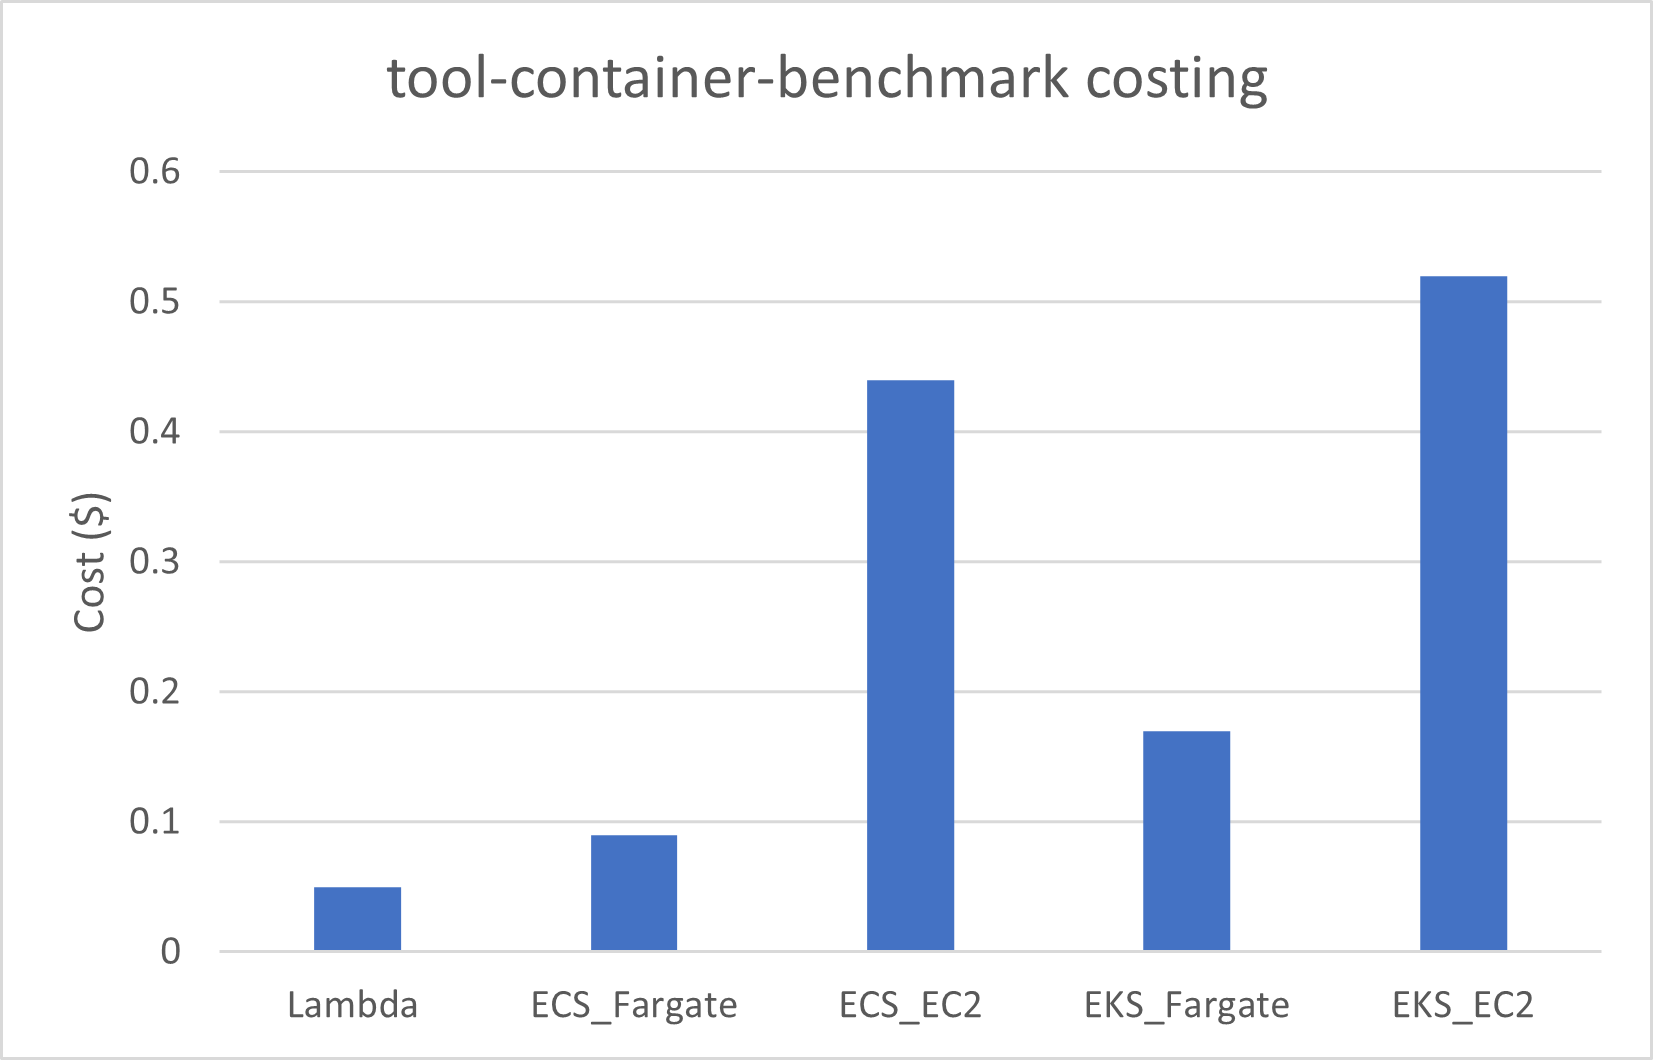
\includegraphics{images/cost-workload.png}
  \caption{\emph{Cost}: Average cost of running \emph{tool-container-benchmark} with 30000 events}
  \label{fig:cost_workload}
\end{figure}

\begin{table}[hp]
  \caption{\emph{Cost}: Projected costing (\$) of running a sample long-lived service per solution for a month and year}
  \small
  \begin{tabularx}{1\textwidth}{X | X | X }
    \space            & \bf{Monthly} & \bf{Annually} \\
    \hline
    \bf{Lambda      } & 120.11       & 1441.32       \\
    \bf{ECS\_Fargate} & 40.99        & 491.88        \\
    \bf{ECS\_EC2    } & 40.623125    & 487.4775      \\
    \bf{EKS\_Fargate} & 113.99       & 1367.88       \\
    \bf{EKS\_EC2    } & 113.623125   & 1363.4775     \\
  \end{tabularx}
  \label{fig:cost_projected}
\end{table}

\begin{figure}[hp]
  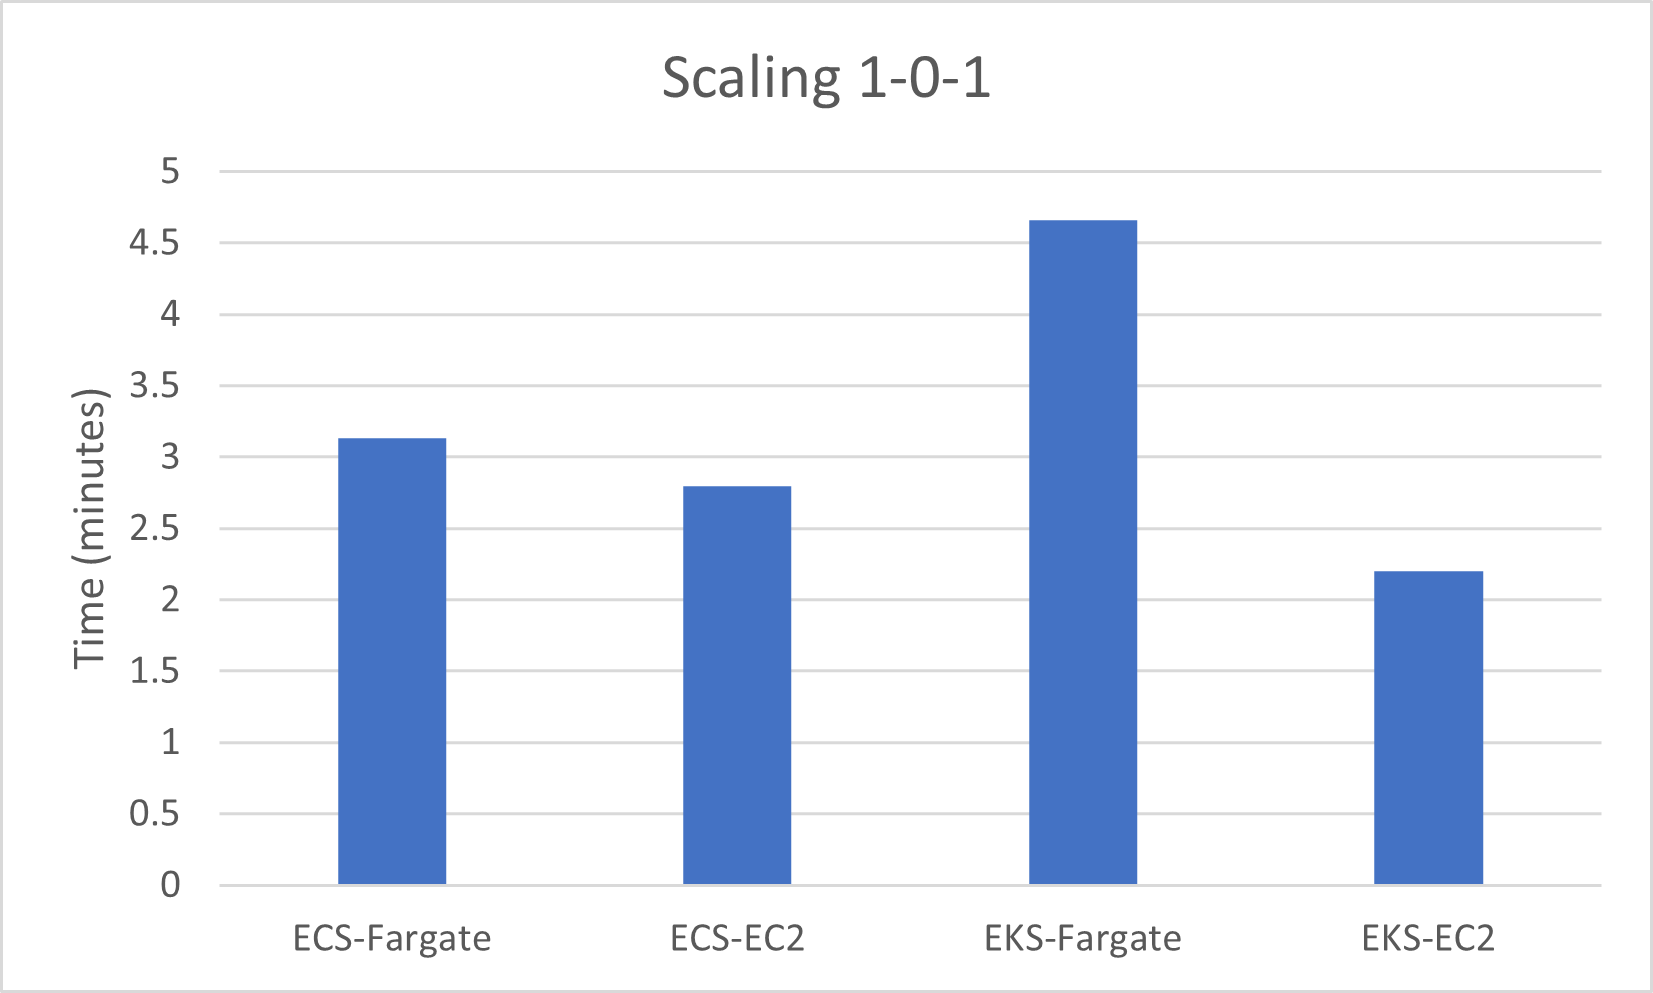
\includegraphics{images/rr-scaling.png}
  \caption{\emph{Resilience and Reliability}: Average amount of downtime measured between scaling operations from one instance, to no instances, and back to one instance}
  \label{fig:rr_scaling}
\end{figure}

\begin{figure}[hp]
  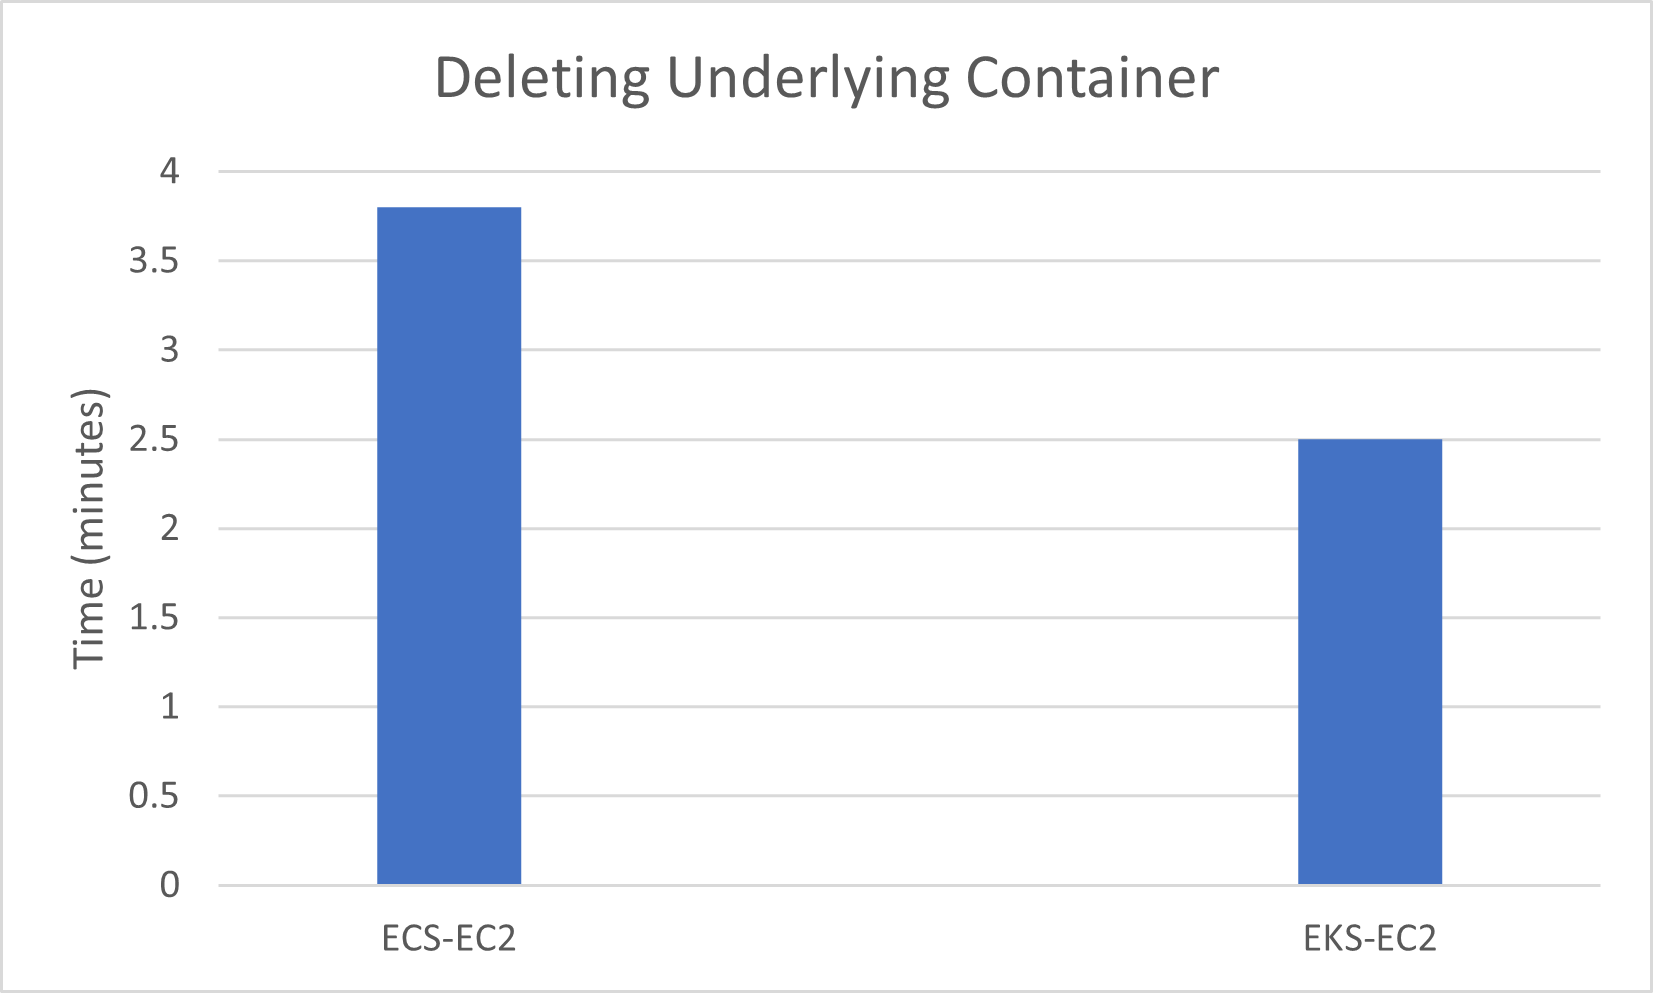
\includegraphics{images/rr-deleteContainer.png}
  \caption{\emph{Resilience and Reliability}: Average amount of downtime measured between deleting a container on underlying host and creation of new container instance}
  \label{fig:rr_deleteContainer}
\end{figure}

\begin{figure}[hp]
  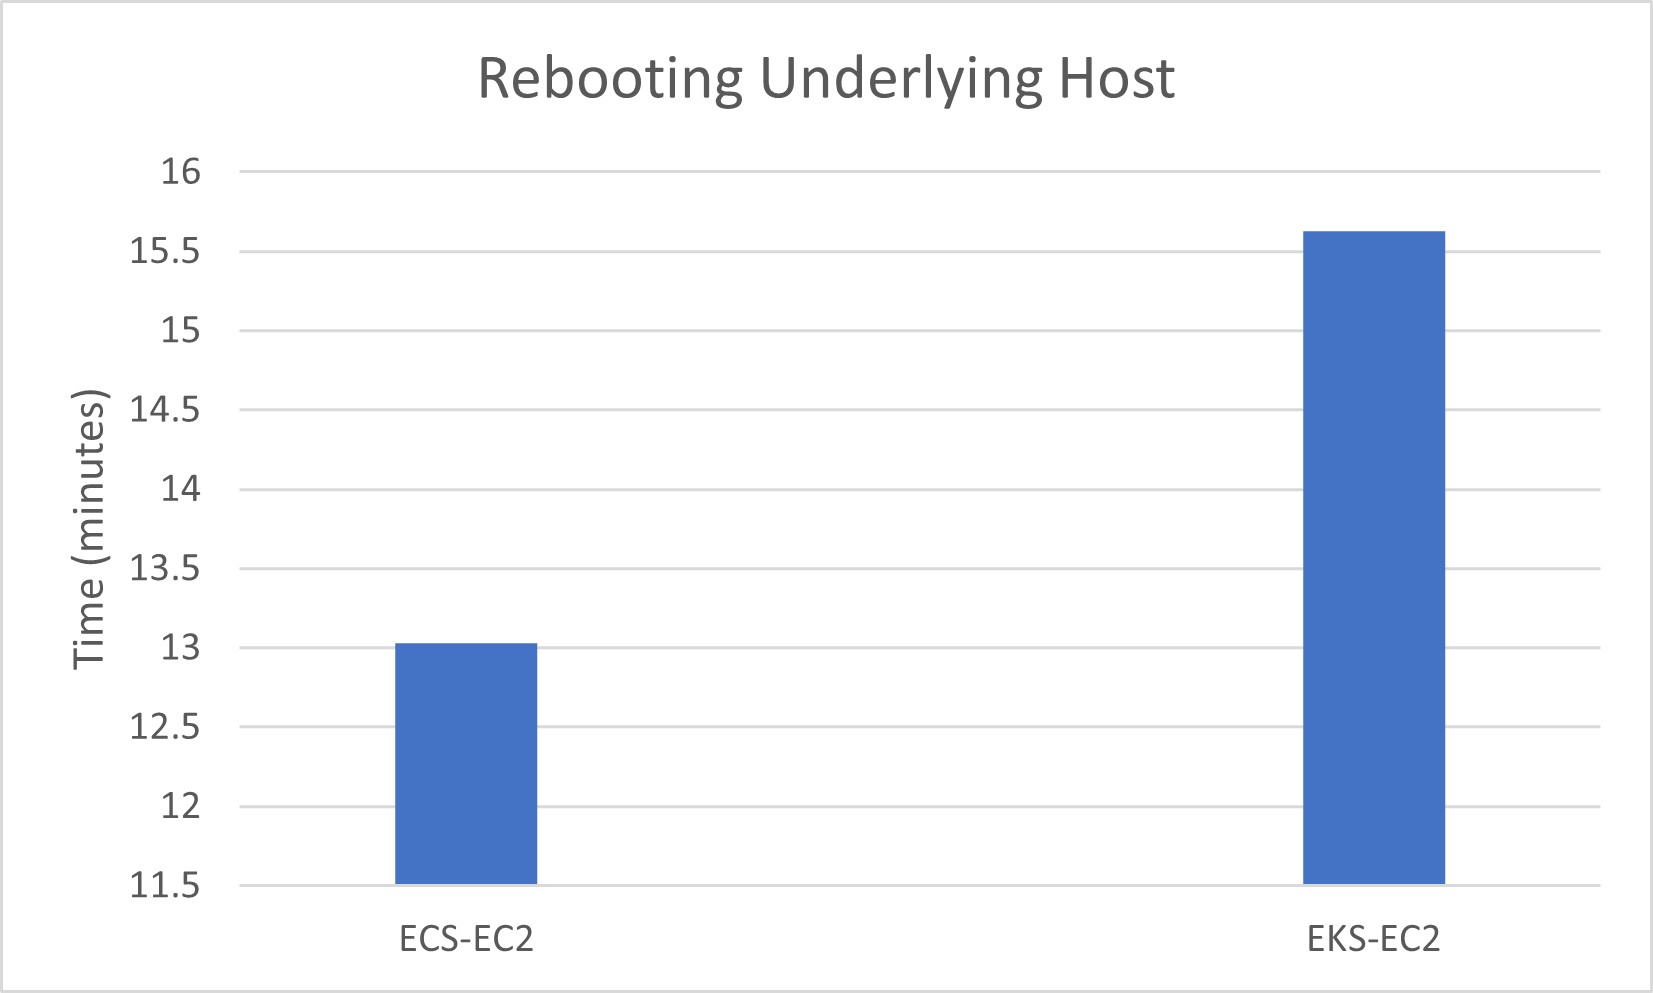
\includegraphics{images/rr-reboot.png}
  \caption{\emph{Resilience and Reliability}: Average amount of downtime measured between deleting a container on underlying host and creation of new container instance}
  \label{fig:rr_reboot}
\end{figure}

\begin{figure}[hp]
  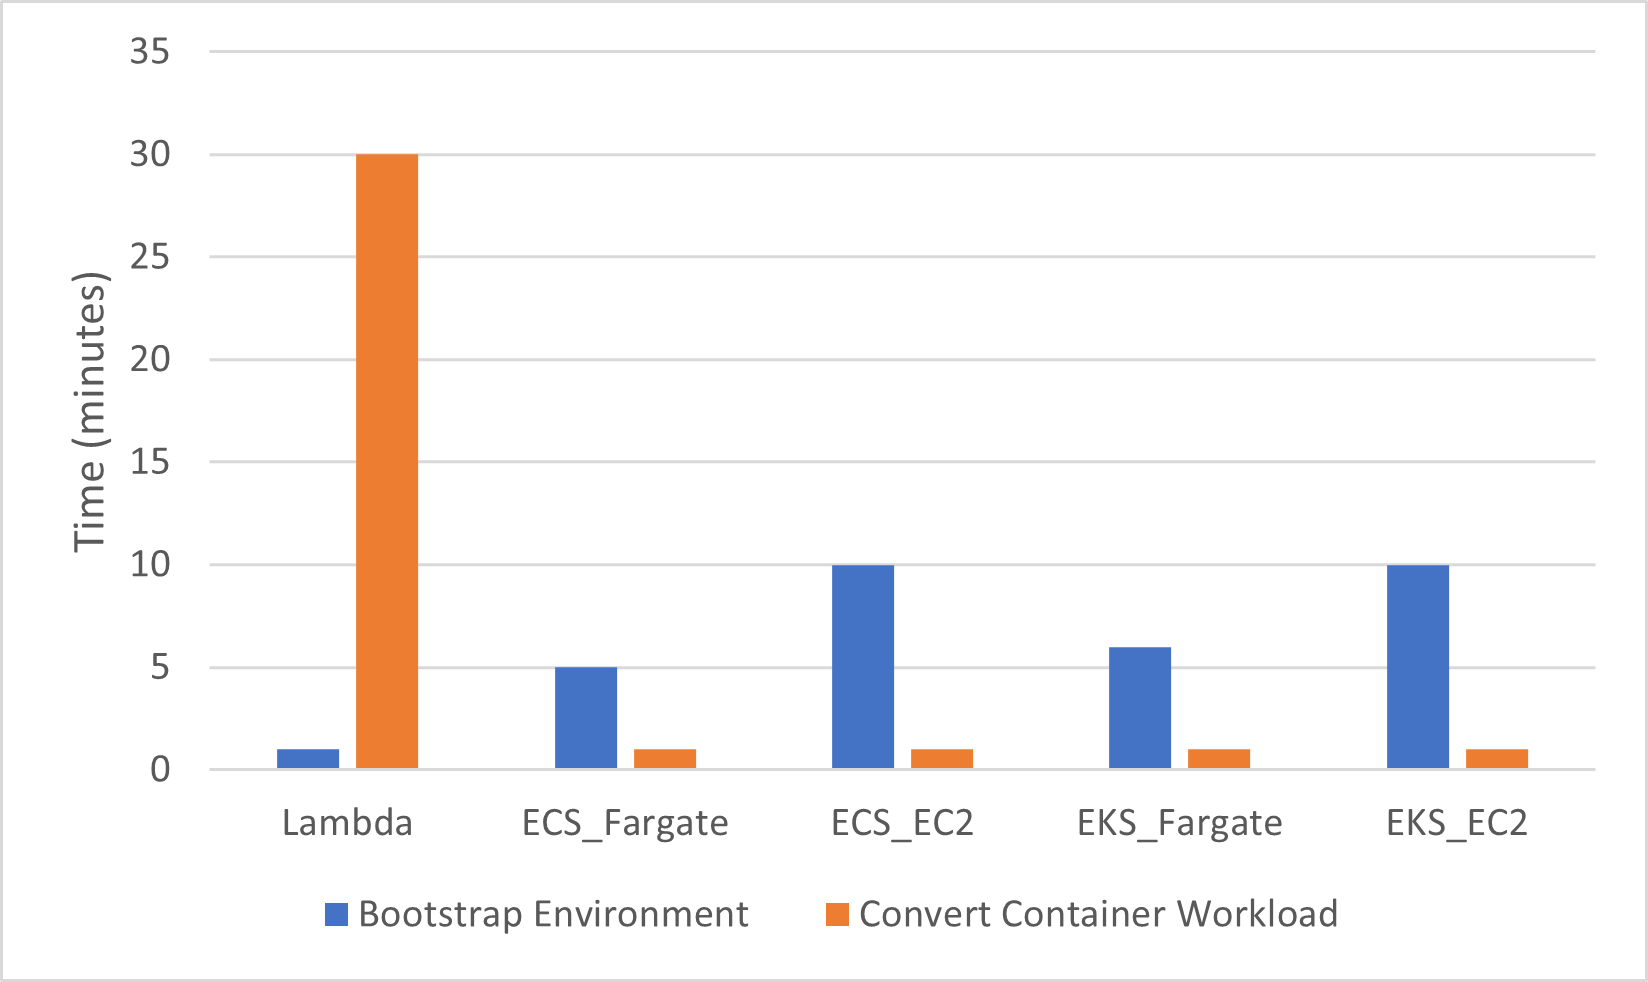
\includegraphics{images/eou.png}
  \caption{\emph{Ease-of-Use}: Amount of time taken to complete environmental bootstrap and convert an existing container workload to run on solution}
  \label{fig:eou}
\end{figure}
